%% ============================================================
%%  Lunar Surface Thermal Model — Plain-Language Summary
%%  Compile with: pdflatex main.tex  (twice for references)
%% ============================================================
\documentclass[12pt, a4paper]{article}

% ── Packages ─────────────────────────────────────────────────
\usepackage[margin=2.5cm]{geometry}
\usepackage{graphicx}
\usepackage{amsmath, amssymb}
\usepackage{booktabs}
\usepackage{caption}
\usepackage{subcaption}
\usepackage{hyperref}
\usepackage{xcolor}
\usepackage{parskip}       % space between paragraphs instead of indent
\usepackage{microtype}
\usepackage{enumitem}
\usepackage{float}

\hypersetup{
  colorlinks = true,
  linkcolor  = blue!60!black,
  citecolor  = blue!60!black,
  urlcolor   = blue!60!black,
}

% ── Custom colours ───────────────────────────────────────────
\definecolor{boxgray}{gray}{0.93}
\definecolor{physicsblue}{RGB}{30, 90, 160}

% ── Simple shaded box for key equations ──────────────────────
\newcommand{\eqbox}[1]{%
  \begin{center}
    \colorbox{boxgray}{\parbox{0.88\linewidth}{\vspace{4pt}\centering#1\vspace{4pt}}}
  \end{center}
}

% ─────────────────────────────────────────────────────────────
\title{%
  \textbf{How Hot Is the Moon Underfoot?}\\[0.4em]
  \large A Plain-Language Guide to the Lunar Surface Thermal Model\\[0.2em]
  \normalsize Apollo Heat-Flow Validation and Geothermal Estimation
}
\author{Lunar Thermal Modelling Project}
\date{March 2026}
% ─────────────────────────────────────────────────────────────

\begin{document}
\maketitle
\tableofcontents
\newpage

%% ============================================================
\section{Why Model the Moon's Temperature?}
%% ============================================================

The Moon has no atmosphere, no ocean, and no weather.  Its surface is exposed
directly to the Sun for a continuous 14-day ``day'' (temperatures can reach
120\,\textdegree{}C), then plunges into a 14-day night where the surface falls
to about $-173$\,\textdegree{}C.

Despite these extreme swings, just \textbf{one metre underground the temperature
barely changes at all}.  That is the key physical insight: the Sun's daily heating
wave can only penetrate a short distance before it is damped out.

Measuring how that temperature wave decays with depth tells us:
\begin{itemize}
  \item What the lunar dust (``regolith'') is made of and how tightly it is packed.
  \item How much heat is escaping from the Moon's interior (geothermal heat flow).
  \item How to design future lunar habitats and instruments.
\end{itemize}

This document describes a 1-D numerical model that simulates this process, and
validates it against data collected by NASA's Apollo~15 and Apollo~17 missions.

%% ============================================================
\section{The Physics in One Equation}
%% ============================================================

Heat conduction through the ground is governed by a single partial differential
equation:

\eqbox{
  $\displaystyle
    \rho(z)\, c(T)\,\frac{\partial T}{\partial t}
    \;=\;
    \frac{\partial}{\partial z}\!\left[k(T,z)\,\frac{\partial T}{\partial z}\right]$
}

\noindent In words:

\begin{center}
\begin{tabular}{clcl}
  $\rho(z)$ & density of the dust (kg/m$^3$) & $\times$ & changes with depth $z$ \\
  $c(T)$    & heat capacity (J/kg/K)          & $\times$ & changes with temperature $T$ \\
  $\partial T/\partial t$ & rate of temperature change & $=$ & \\
  $\partial/\partial z[\cdots]$ & \multicolumn{3}{l}{net heat flowing in minus heat flowing out at each layer}
\end{tabular}
\end{center}

\vspace{0.5em}
The key material property is the \textbf{thermal conductivity} $k$ (W/m/K),
which controls how easily heat flows through the material.  For lunar dust,
heat moves in two ways:
\begin{enumerate}
  \item \textbf{Contact conduction}: dust grains touch each other and pass heat
        like a chain of hands.  This dominates at cold temperatures.
  \item \textbf{Radiative conduction}: each grain glows infrared light and
        ``sees'' its neighbours.  This grows as $T^3$ and dominates at hot
        dayside temperatures.
\end{enumerate}
Together:
\eqbox{
  $k_{\text{total}}(T,z) = k_{\text{solid}}(z)\;\left[1 + \chi\!\left(\dfrac{T}{350\,\text{K}}\right)^{\!3}\right]$
}

\noindent where $\chi = 2.7$ is the radiative coefficient (Hayne et al.\ 2017)
and $350\,\text{K}$ is a reference temperature.

%% ============================================================
\section{The Two Dust Models}
%% ============================================================

We do not know the exact density and conductivity of lunar dust at every depth,
so we test two published models calibrated to different data sets.

\subsection{Discrete Layers (Apollo drill cores, Carrier et al.\ 1991)}

Apollo astronauts drilled into the surface and extracted core samples.  These
revealed a distinct layered structure:

\begin{center}
\begin{tabular}{lll}
  \toprule
  Depth range & Bulk density & Physical description \\
  \midrule
  0 -- 7\,cm  & 1100\,kg/m$^3$ & Very fluffy surface dust; newly deposited \\
  7 -- 20\,cm & increasing    & Transition; dust compacted by micrometeorites \\
  $>$20\,cm   & 1700\,kg/m$^3$ & Compacted regolith \\
  \bottomrule
\end{tabular}
\end{center}

The solid conductivity ranges from $k_{\text{solid}} = 1.0$\,mW/m/K at the
surface to $6.3$\,mW/m/K at depth (calibrated to Apollo heat-flow probe
gradient measurements; Langseth et al.\ 1976).

\subsection{Exponential Profile (Hayne et al.\ 2017, Diviner satellite)}

NASA's Lunar Reconnaissance Orbiter carries the Diviner radiometer, which
measures surface temperatures globally from orbit.  Hayne et al.\ (2017) fitted
these data with a smooth exponential density increase:

\eqbox{
  $\rho(z) = \rho_d - (\rho_d - \rho_s)\,e^{-z/H}$
}

\noindent with $\rho_s = 1100$\,kg/m$^3$ (surface), $\rho_d = 1800$\,kg/m$^3$
(deep), and scale height $H = 7$\,cm.  Conductivity follows the same profile:
$k_{\text{solid}}$ rises smoothly from $0.74$\,mW/m/K to $3.8$\,mW/m/K.

\medskip
The two models agree well in the top 20\,cm but differ at depth, reflecting
that Diviner is sensitive to the thermal skin depth ($\sim$5\,cm) while
Apollo probes measured deeper steady-state gradients.

%% ============================================================
\section{Boundary Conditions: How We Drive the Model}
%% ============================================================

\subsection{Top boundary: solar and infrared radiation}

The surface temperature is not prescribed directly.  Instead, the energy
balance is solved at every time step:

\eqbox{
  $Q_{\text{solar}}(t)\,(1-A) + \varepsilon\,\sigma\,T_{\text{sky}}^4
  \;=\; \varepsilon\,\sigma\,T_{\text{surf}}^4 + k\,\frac{\partial T}{\partial z}\bigg|_{z=0}$
}

\begin{itemize}
  \item $Q_{\text{solar}}(t)$ varies with the Moon's rotation (one revolution
        every 29.5 Earth days) and the local slope.
  \item $A = 0.09$ is the surface albedo (reflectivity); lunar dust is dark.
  \item $\varepsilon = 0.95$ is the emissivity (how efficiently the surface
        radiates heat back to space).
  \item $\sigma$ is the Stefan--Boltzmann constant.
\end{itemize}

\subsection{Bottom boundary: geothermal heat from the interior}

At the base of the model column (3\,m depth), heat leaks upward from the
Moon's warm interior:

\eqbox{
  $-k\,\dfrac{\partial T}{\partial z}\bigg|_{\text{base}} = Q_{\text{basal}} = 18\;\text{mW/m}^2$
}

This ``upward heat flux'' boundary condition allows the deep temperature to
float naturally rather than being fixed.

%% ============================================================
\section{The Apollo Heat-Flow Experiment (HFE)}
%% ============================================================

During Apollo~15 (1971) and Apollo~17 (1972), astronauts drilled boreholes
and inserted temperature probes.  The probes took readings for several years
after the astronauts left.

\subsection{Probe equilibration}

The drilling process heated the surrounding rock.  Figure~\ref{fig:equil}
shows how each probe slowly cooled back toward the ambient temperature over
roughly six months.  The final equilibrium values — not the early readings —
are used for model validation.

\begin{figure}[H]
  \centering
  \begin{subfigure}[t]{0.48\textwidth}
    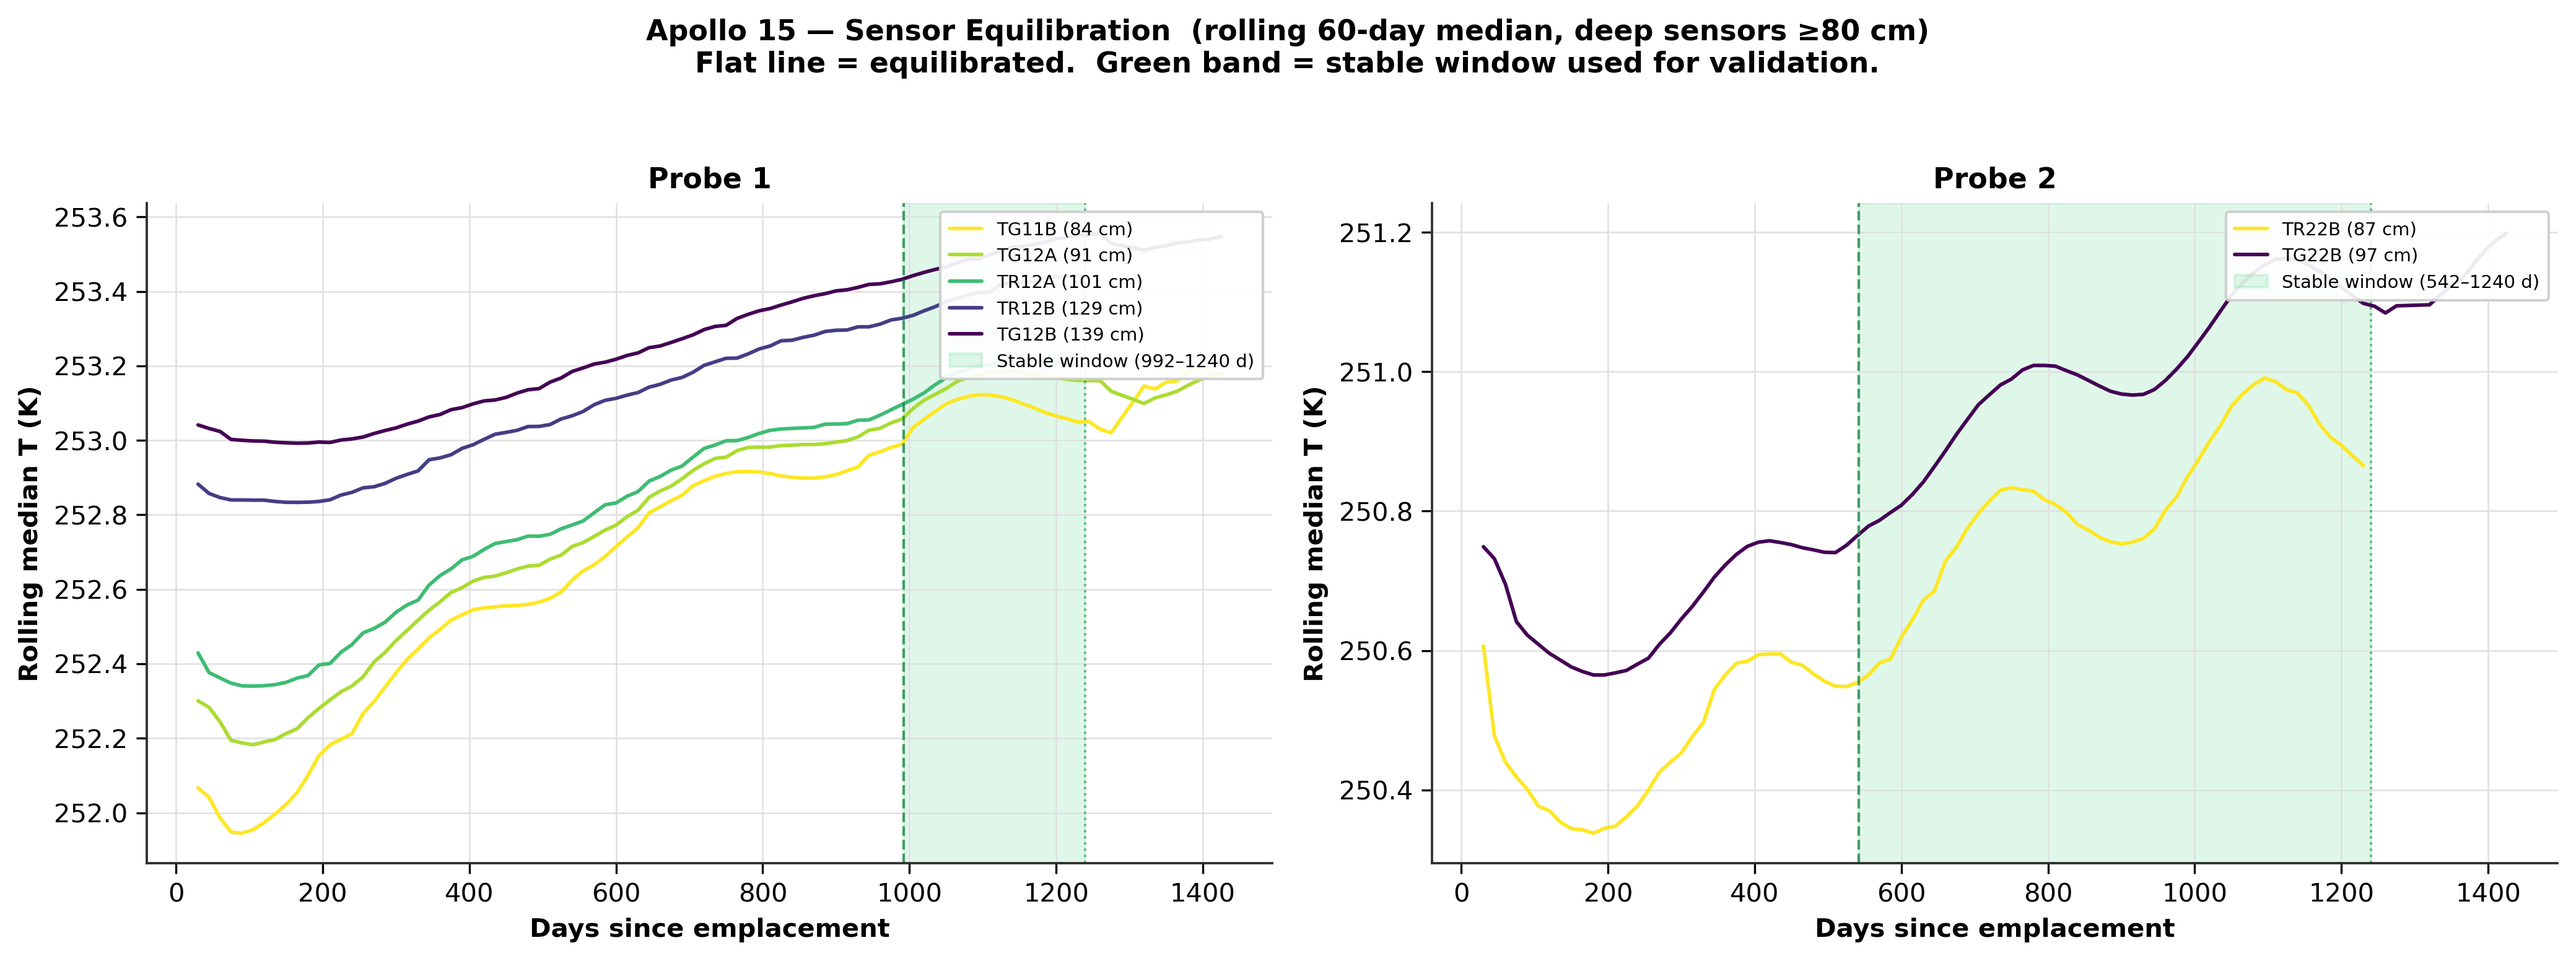
\includegraphics[width=\linewidth]{figures/06_apollo15_equilibration.png}
    \caption{Apollo 15 HFE sensor equilibration.}
  \end{subfigure}\hfill
  \begin{subfigure}[t]{0.48\textwidth}
    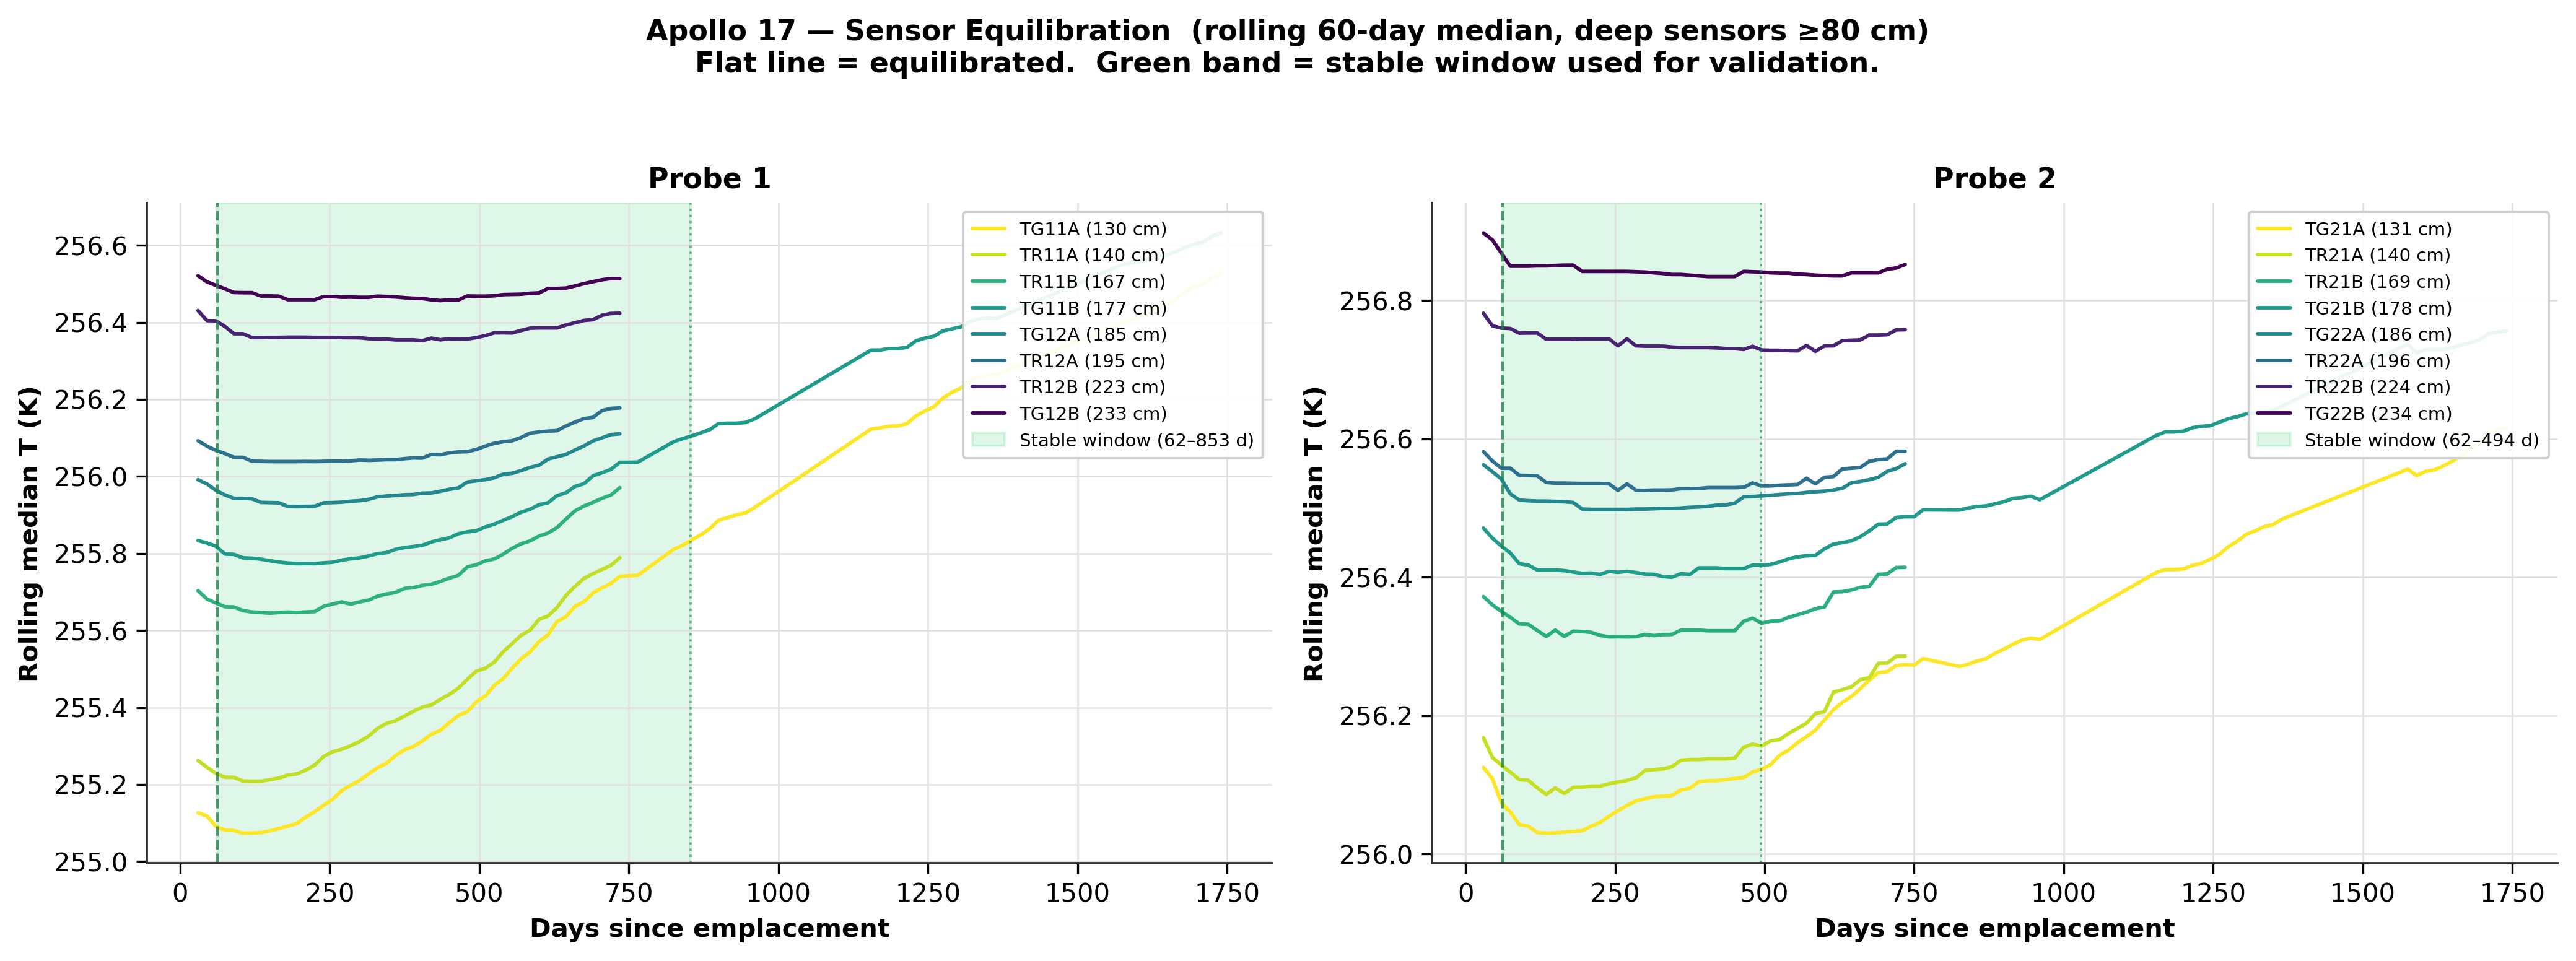
\includegraphics[width=\linewidth]{figures/07_apollo17_equilibration.png}
    \caption{Apollo 17 HFE sensor equilibration.}
  \end{subfigure}
  \caption{Temperature vs.\ time for each HFE thermocouple, showing the
    drilling heat spike and subsequent equilibration.  Dashed lines mark
    the final stable temperatures used for validation.}
  \label{fig:equil}
\end{figure}

\subsection{Sensor selection}

Only sensors at depths $\geq 80$\,cm are used for model comparison.
Shallower sensors are still influenced by the diurnal surface wave and
cannot cleanly measure the deeper, time-invariant geothermal signal.

%% ============================================================
\section{Diurnal Temperature Cycles}
%% ============================================================

Figure~\ref{fig:diurnal} shows the simulated surface temperature over one
full lunar day (29.5 Earth days) at the Apollo~15 site (26\textdegree{}N).

\begin{figure}[H]
  \centering
  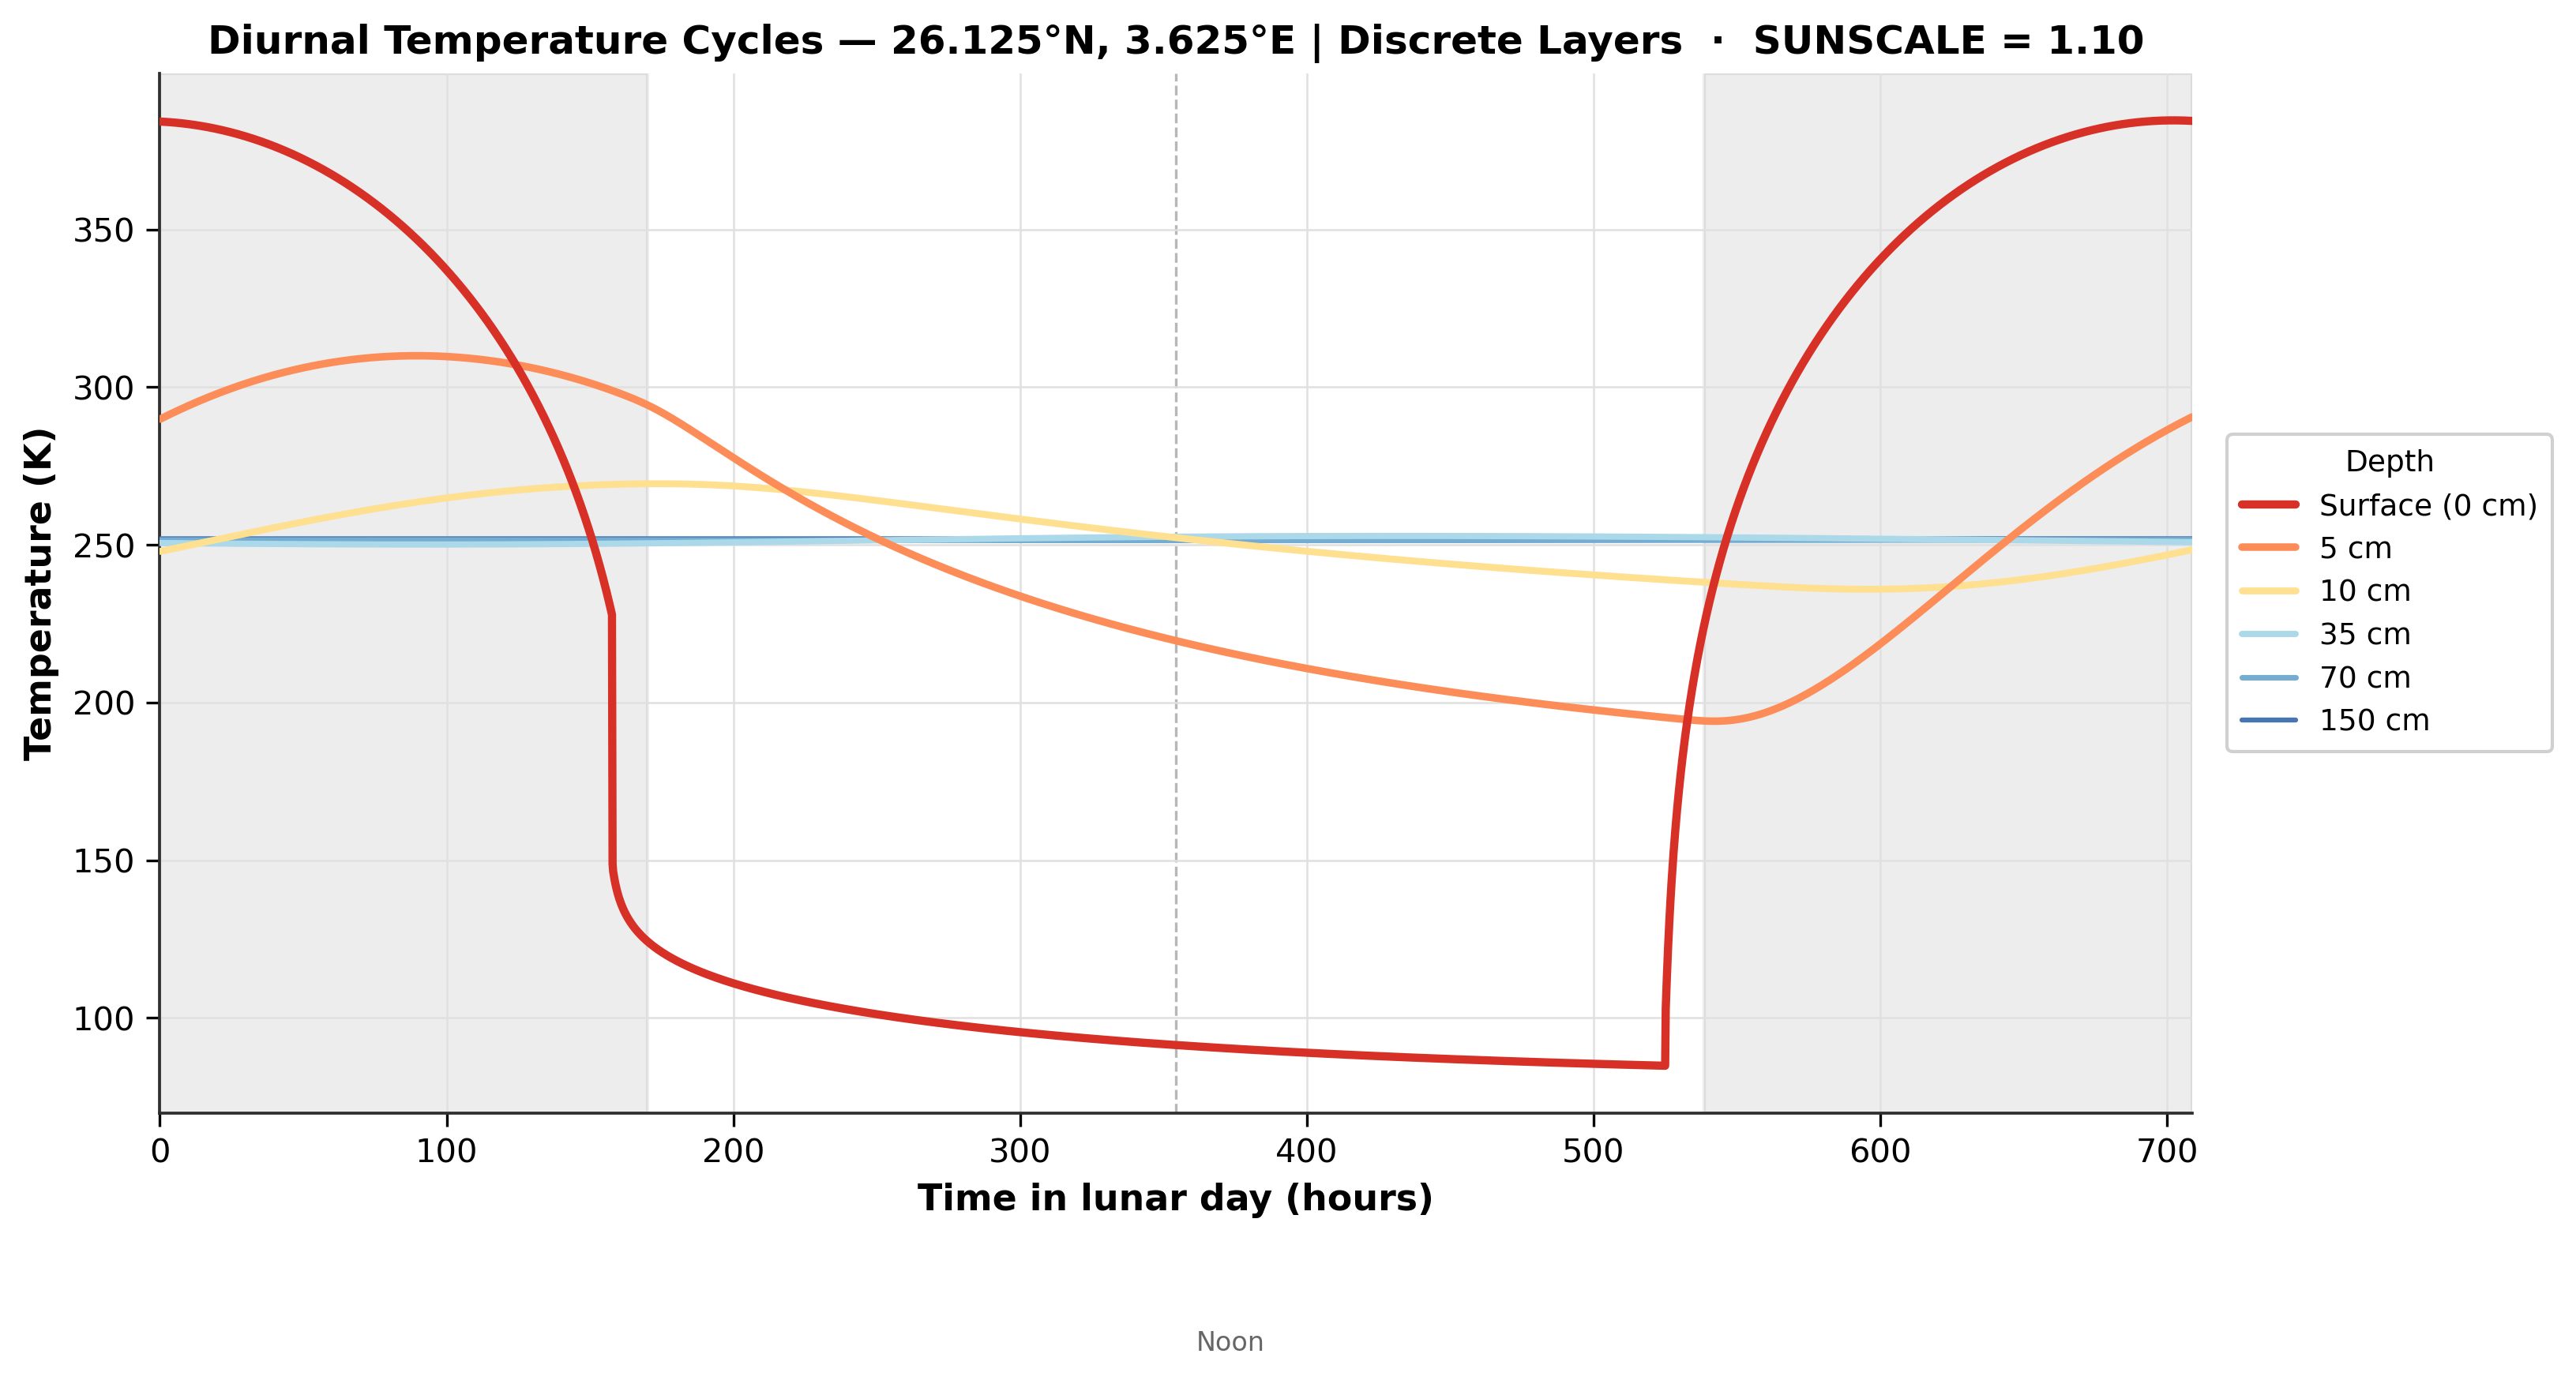
\includegraphics[width=0.85\textwidth]{figures/01_diurnal_cycles.png}
  \caption{Simulated temperature vs.\ local solar time at multiple depths
    (Apollo~15, Discrete model).  The surface oscillates by $\sim$270\,K;
    by 1\,m depth the oscillation is less than 1\,K.}
  \label{fig:diurnal}
\end{figure}

The amplitude decays exponentially with depth over a characteristic
\textbf{thermal skin depth} $\delta$:

\eqbox{
  $\delta = \sqrt{\dfrac{k}{\rho\, c\, \pi / P}}$
}

\noindent where $P$ is the period of the forcing (one lunar day).
For typical lunar surface regolith, $\delta \approx 5$--$10$\,cm.

Figure~\ref{fig:amplitude} shows this exponential decay for both models.
Both collapse to essentially zero amplitude by $\sim$50\,cm, confirming that
deep temperatures are clean indicators of geothermal, not solar, heat.

\begin{figure}[H]
  \centering
  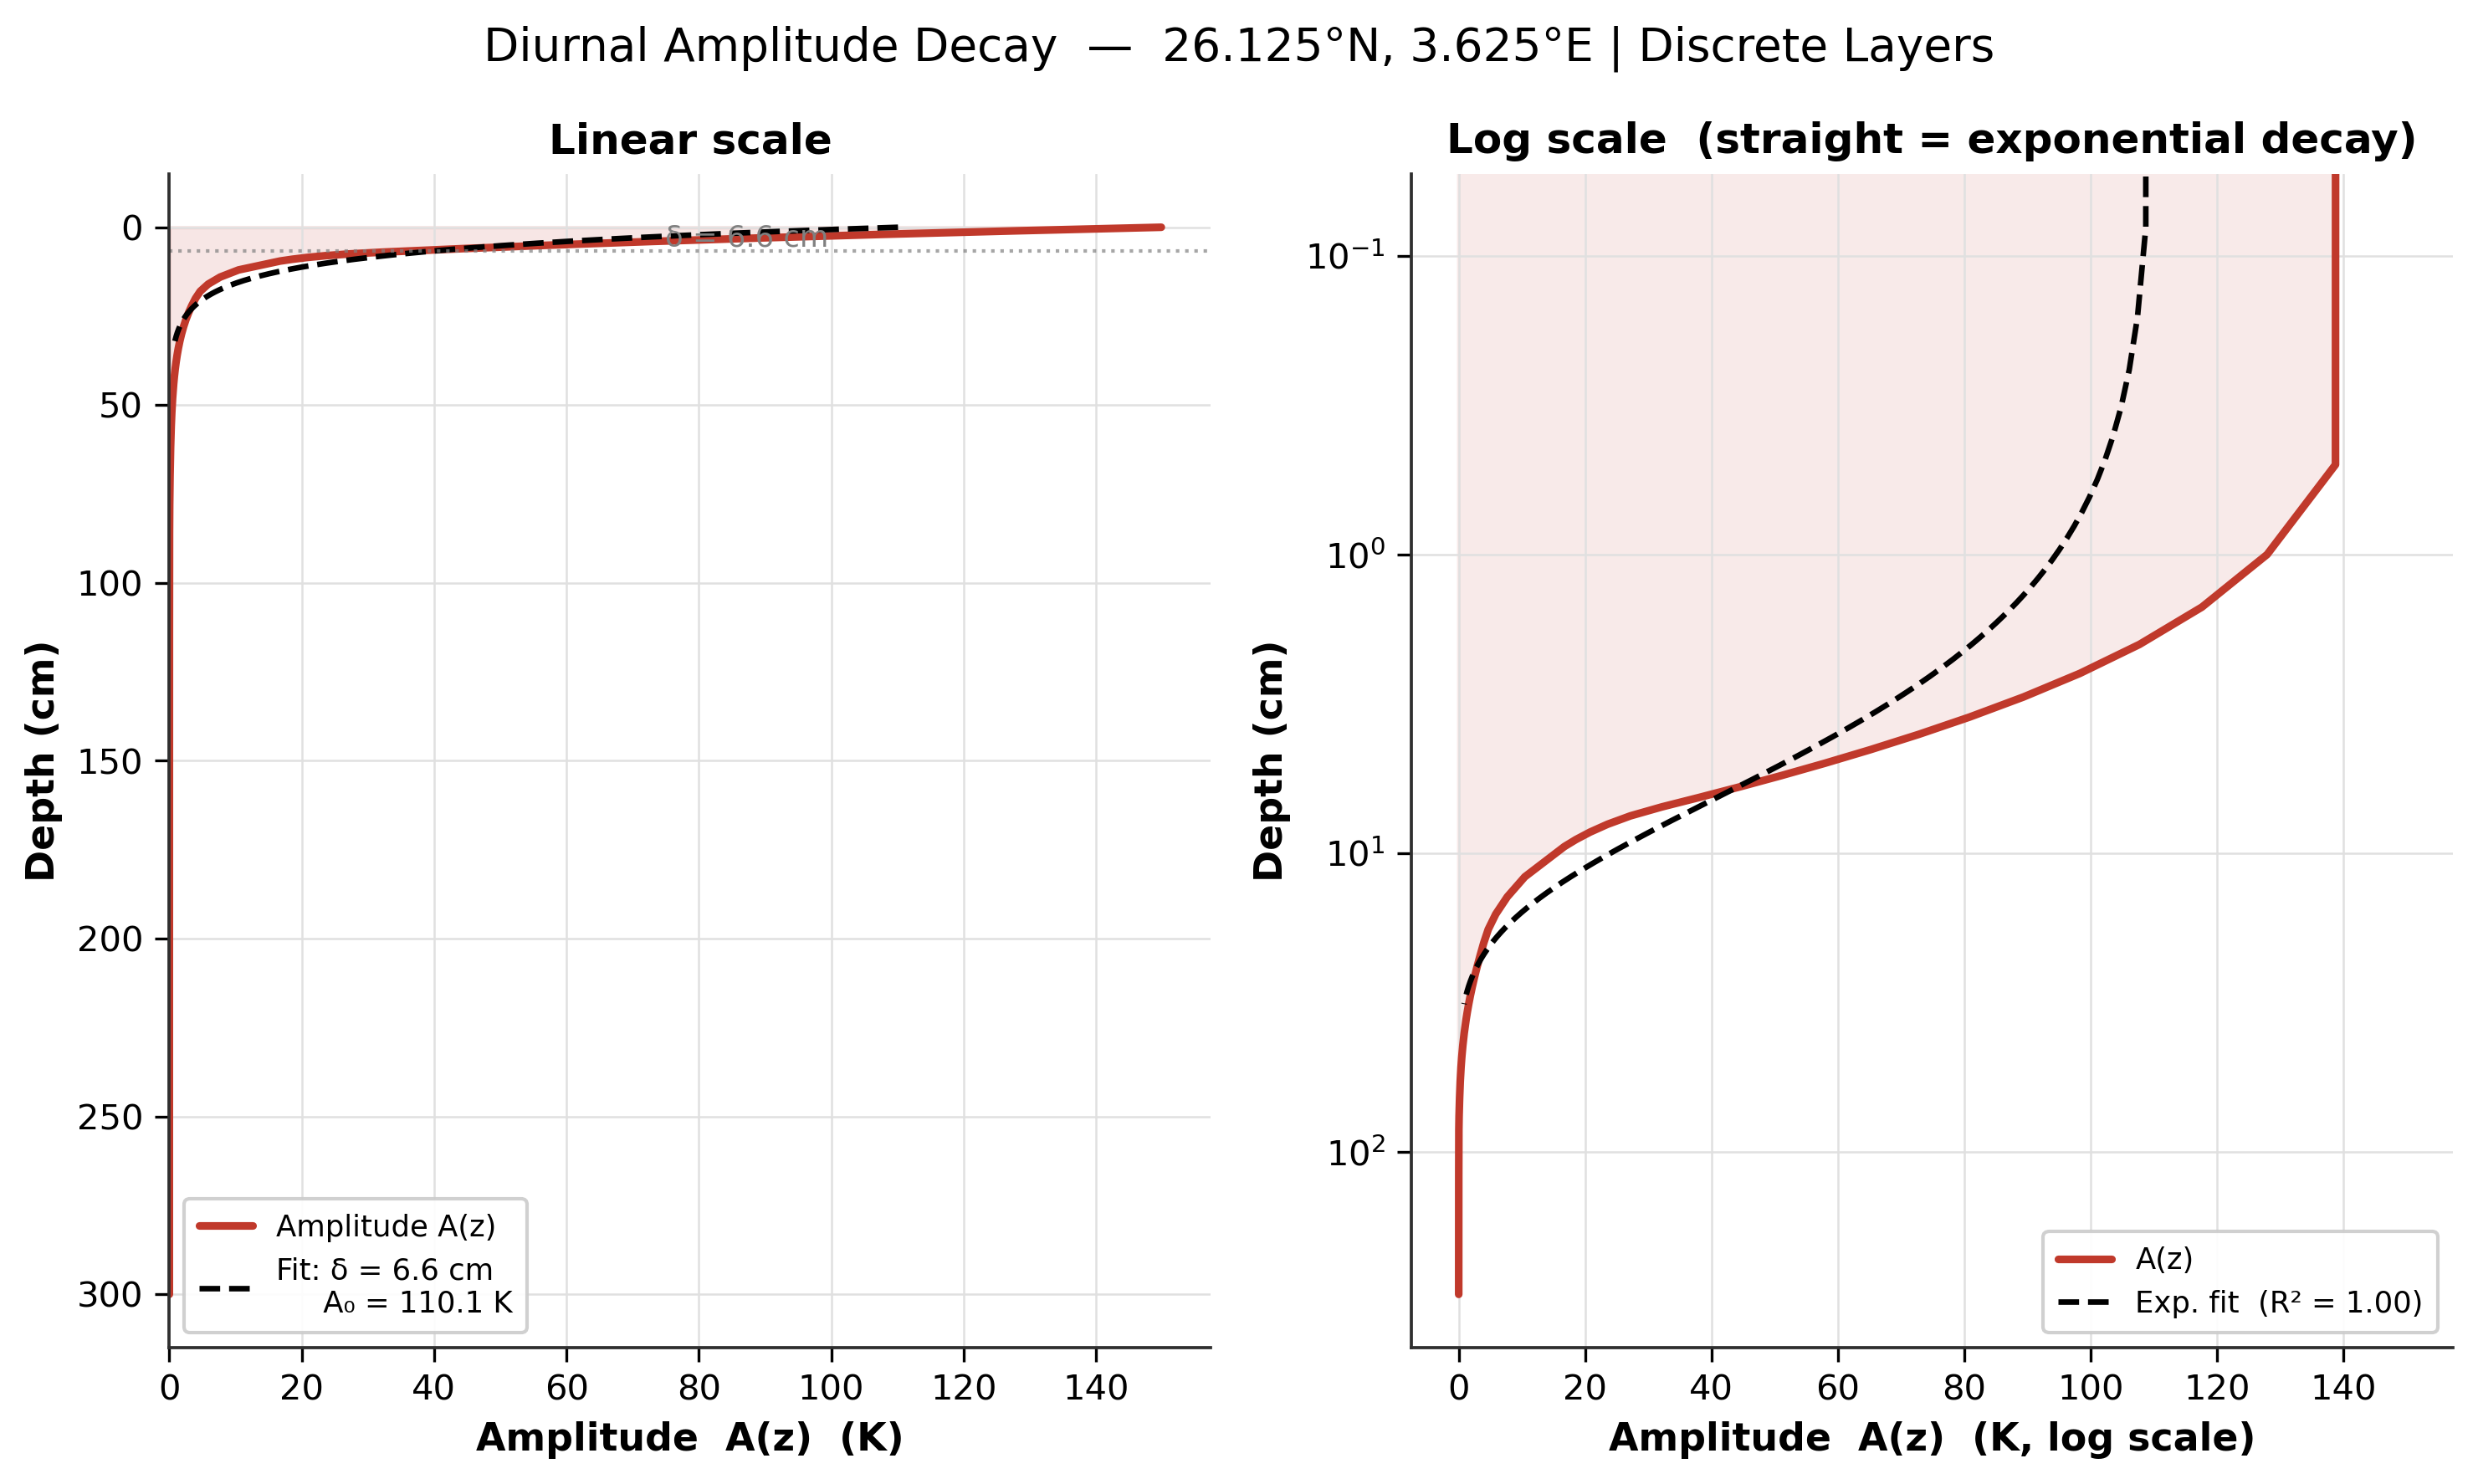
\includegraphics[width=0.70\textwidth]{figures/02_amplitude_decay.png}
  \caption{Diurnal temperature amplitude vs.\ depth for the Discrete and
    Hayne models.  Amplitude decays by four orders of magnitude in the top
    50\,cm.}
  \label{fig:amplitude}
\end{figure}

%% ============================================================
\section{Thermal Properties of the Regolith}
%% ============================================================

Figure~\ref{fig:heatmap} shows the full temperature field as a colour image,
depth on the vertical axis and time on the horizontal axis.

\begin{figure}[H]
  \centering
  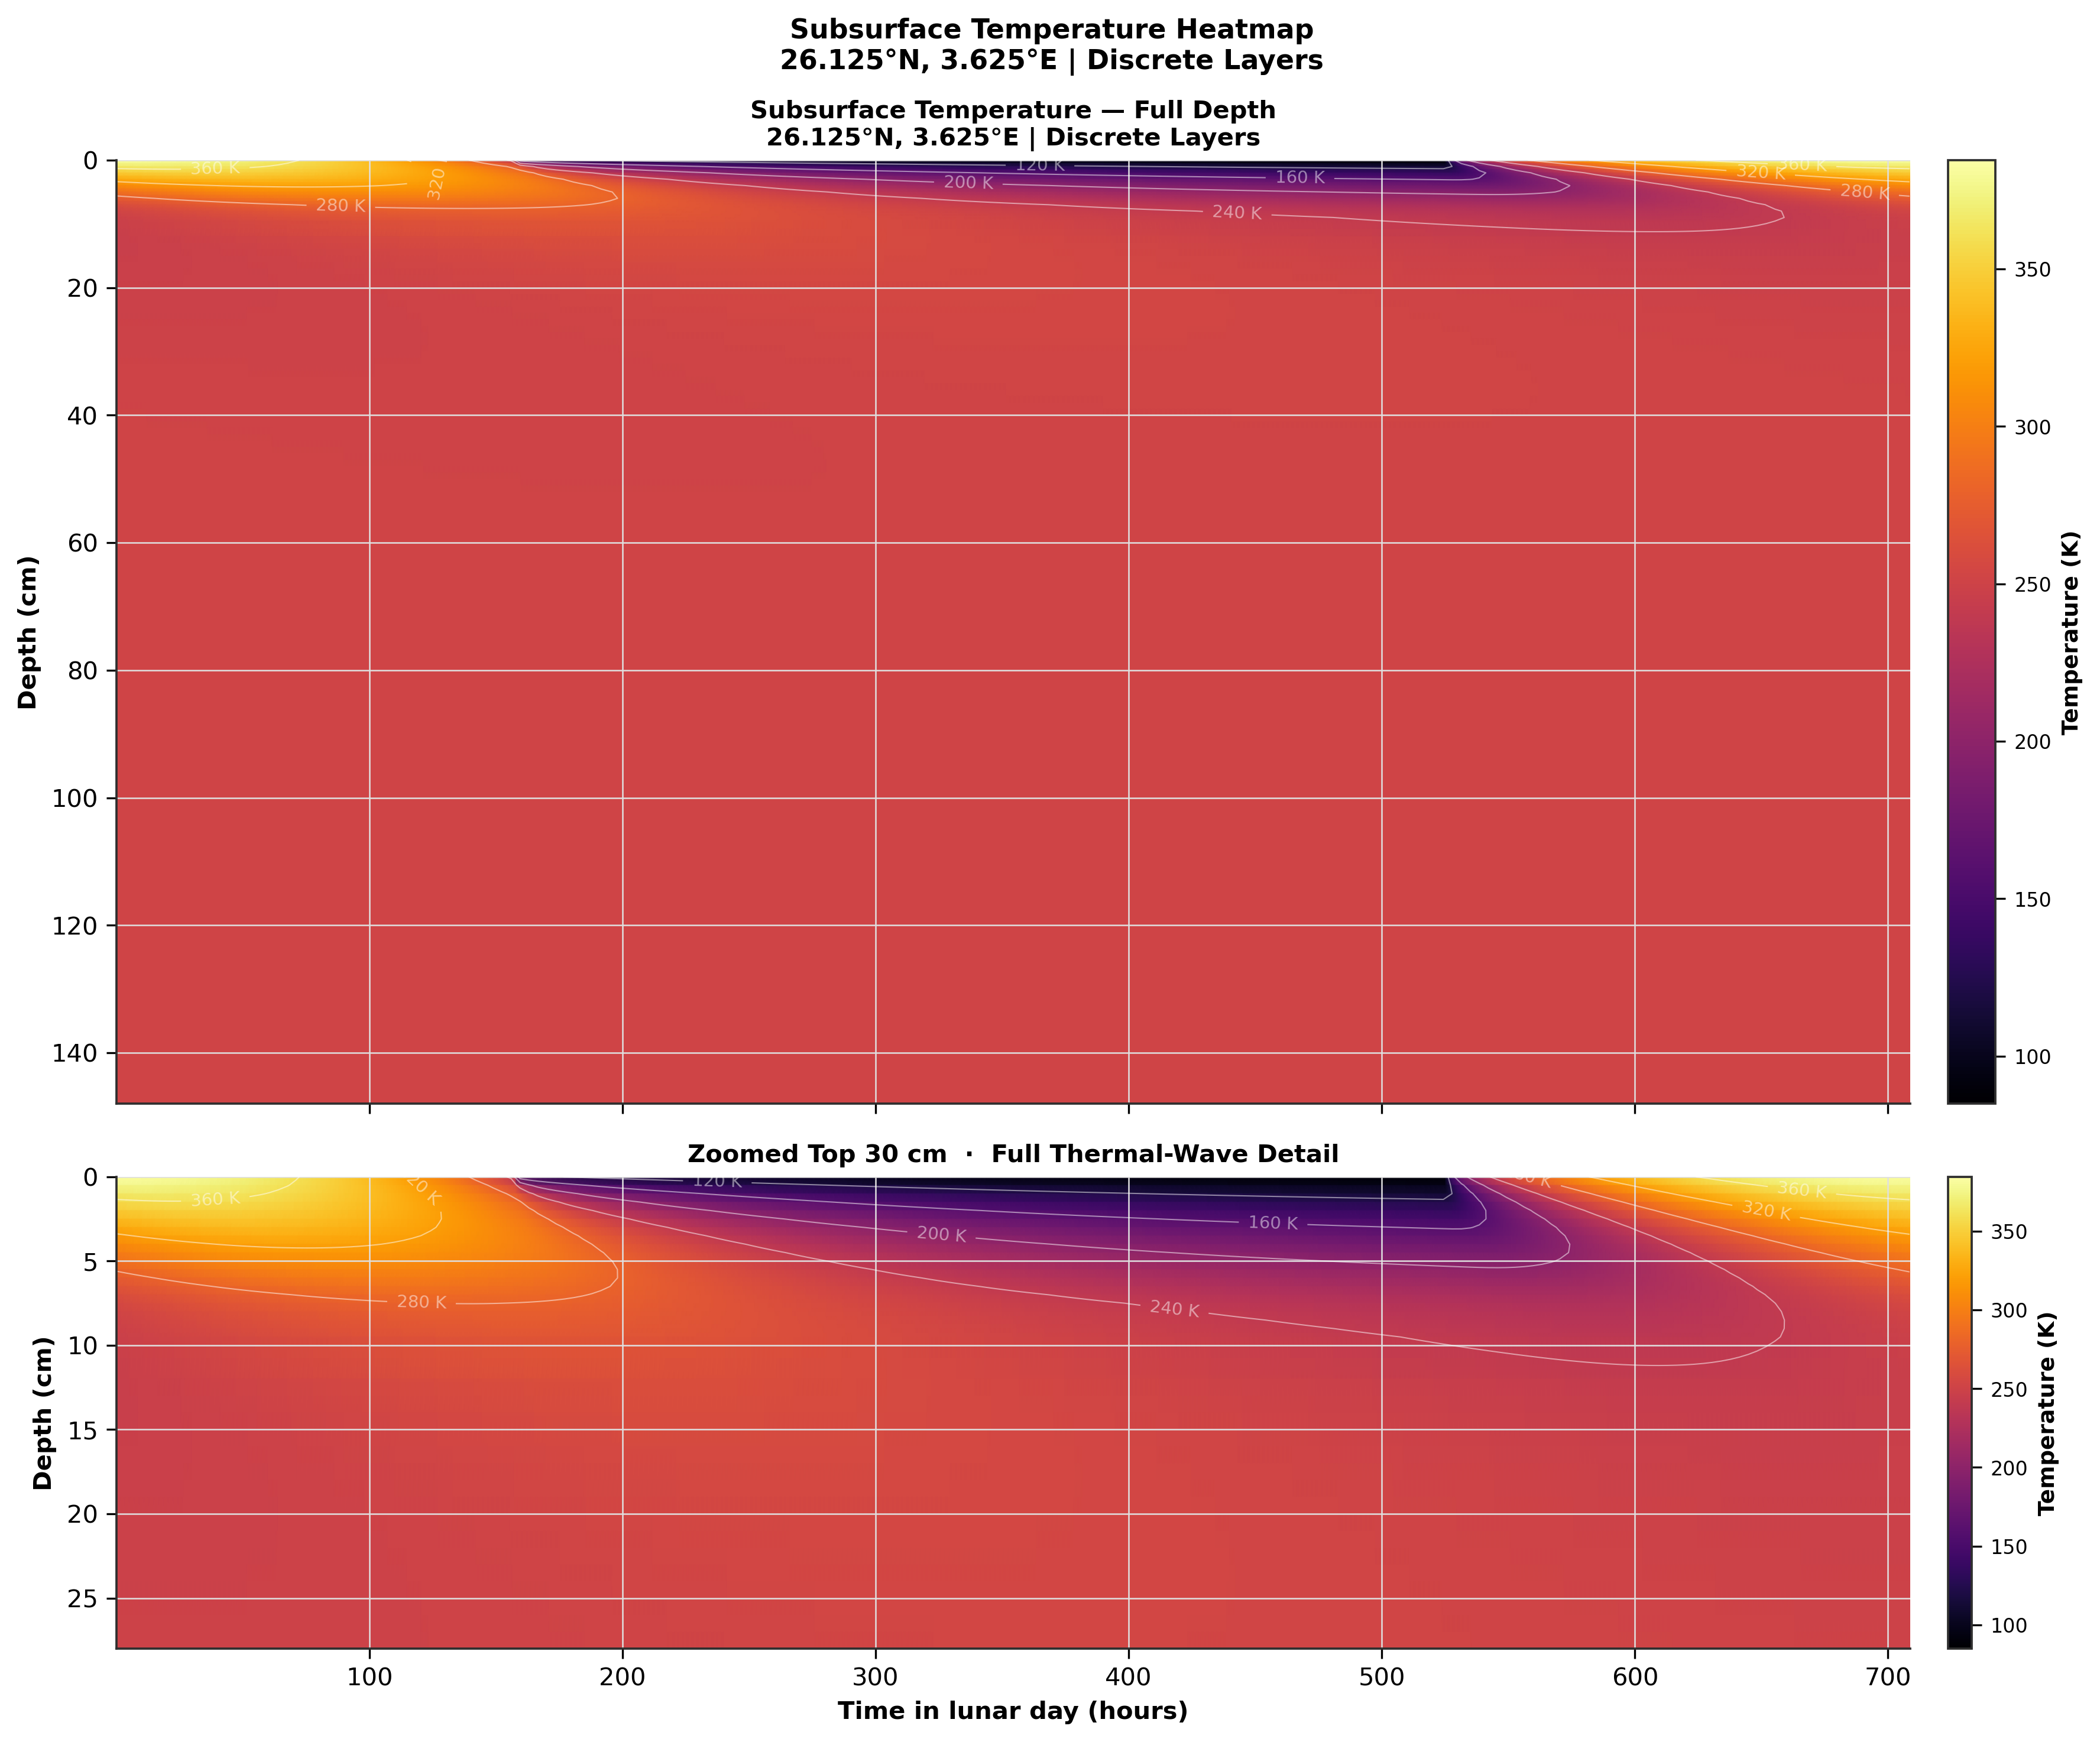
\includegraphics[width=0.85\textwidth]{figures/04_heatmap.png}
  \caption{Temperature heatmap (depth $\times$ time) for one lunar day.
    The yellow ``tongue'' near the surface is the dayside heating pulse.
    Below $\sim$50\,cm the colour is uniform — the deep regolith is
    thermally shielded from the surface.}
  \label{fig:heatmap}
\end{figure}

%% ============================================================
\section{Model vs.\ Apollo Comparison}
%% ============================================================

Figure~\ref{fig:comparison} compares model-predicted mean temperature
profiles against the time-averaged Apollo thermocouple readings for both
sites and both models.

\begin{figure}[H]
  \centering
  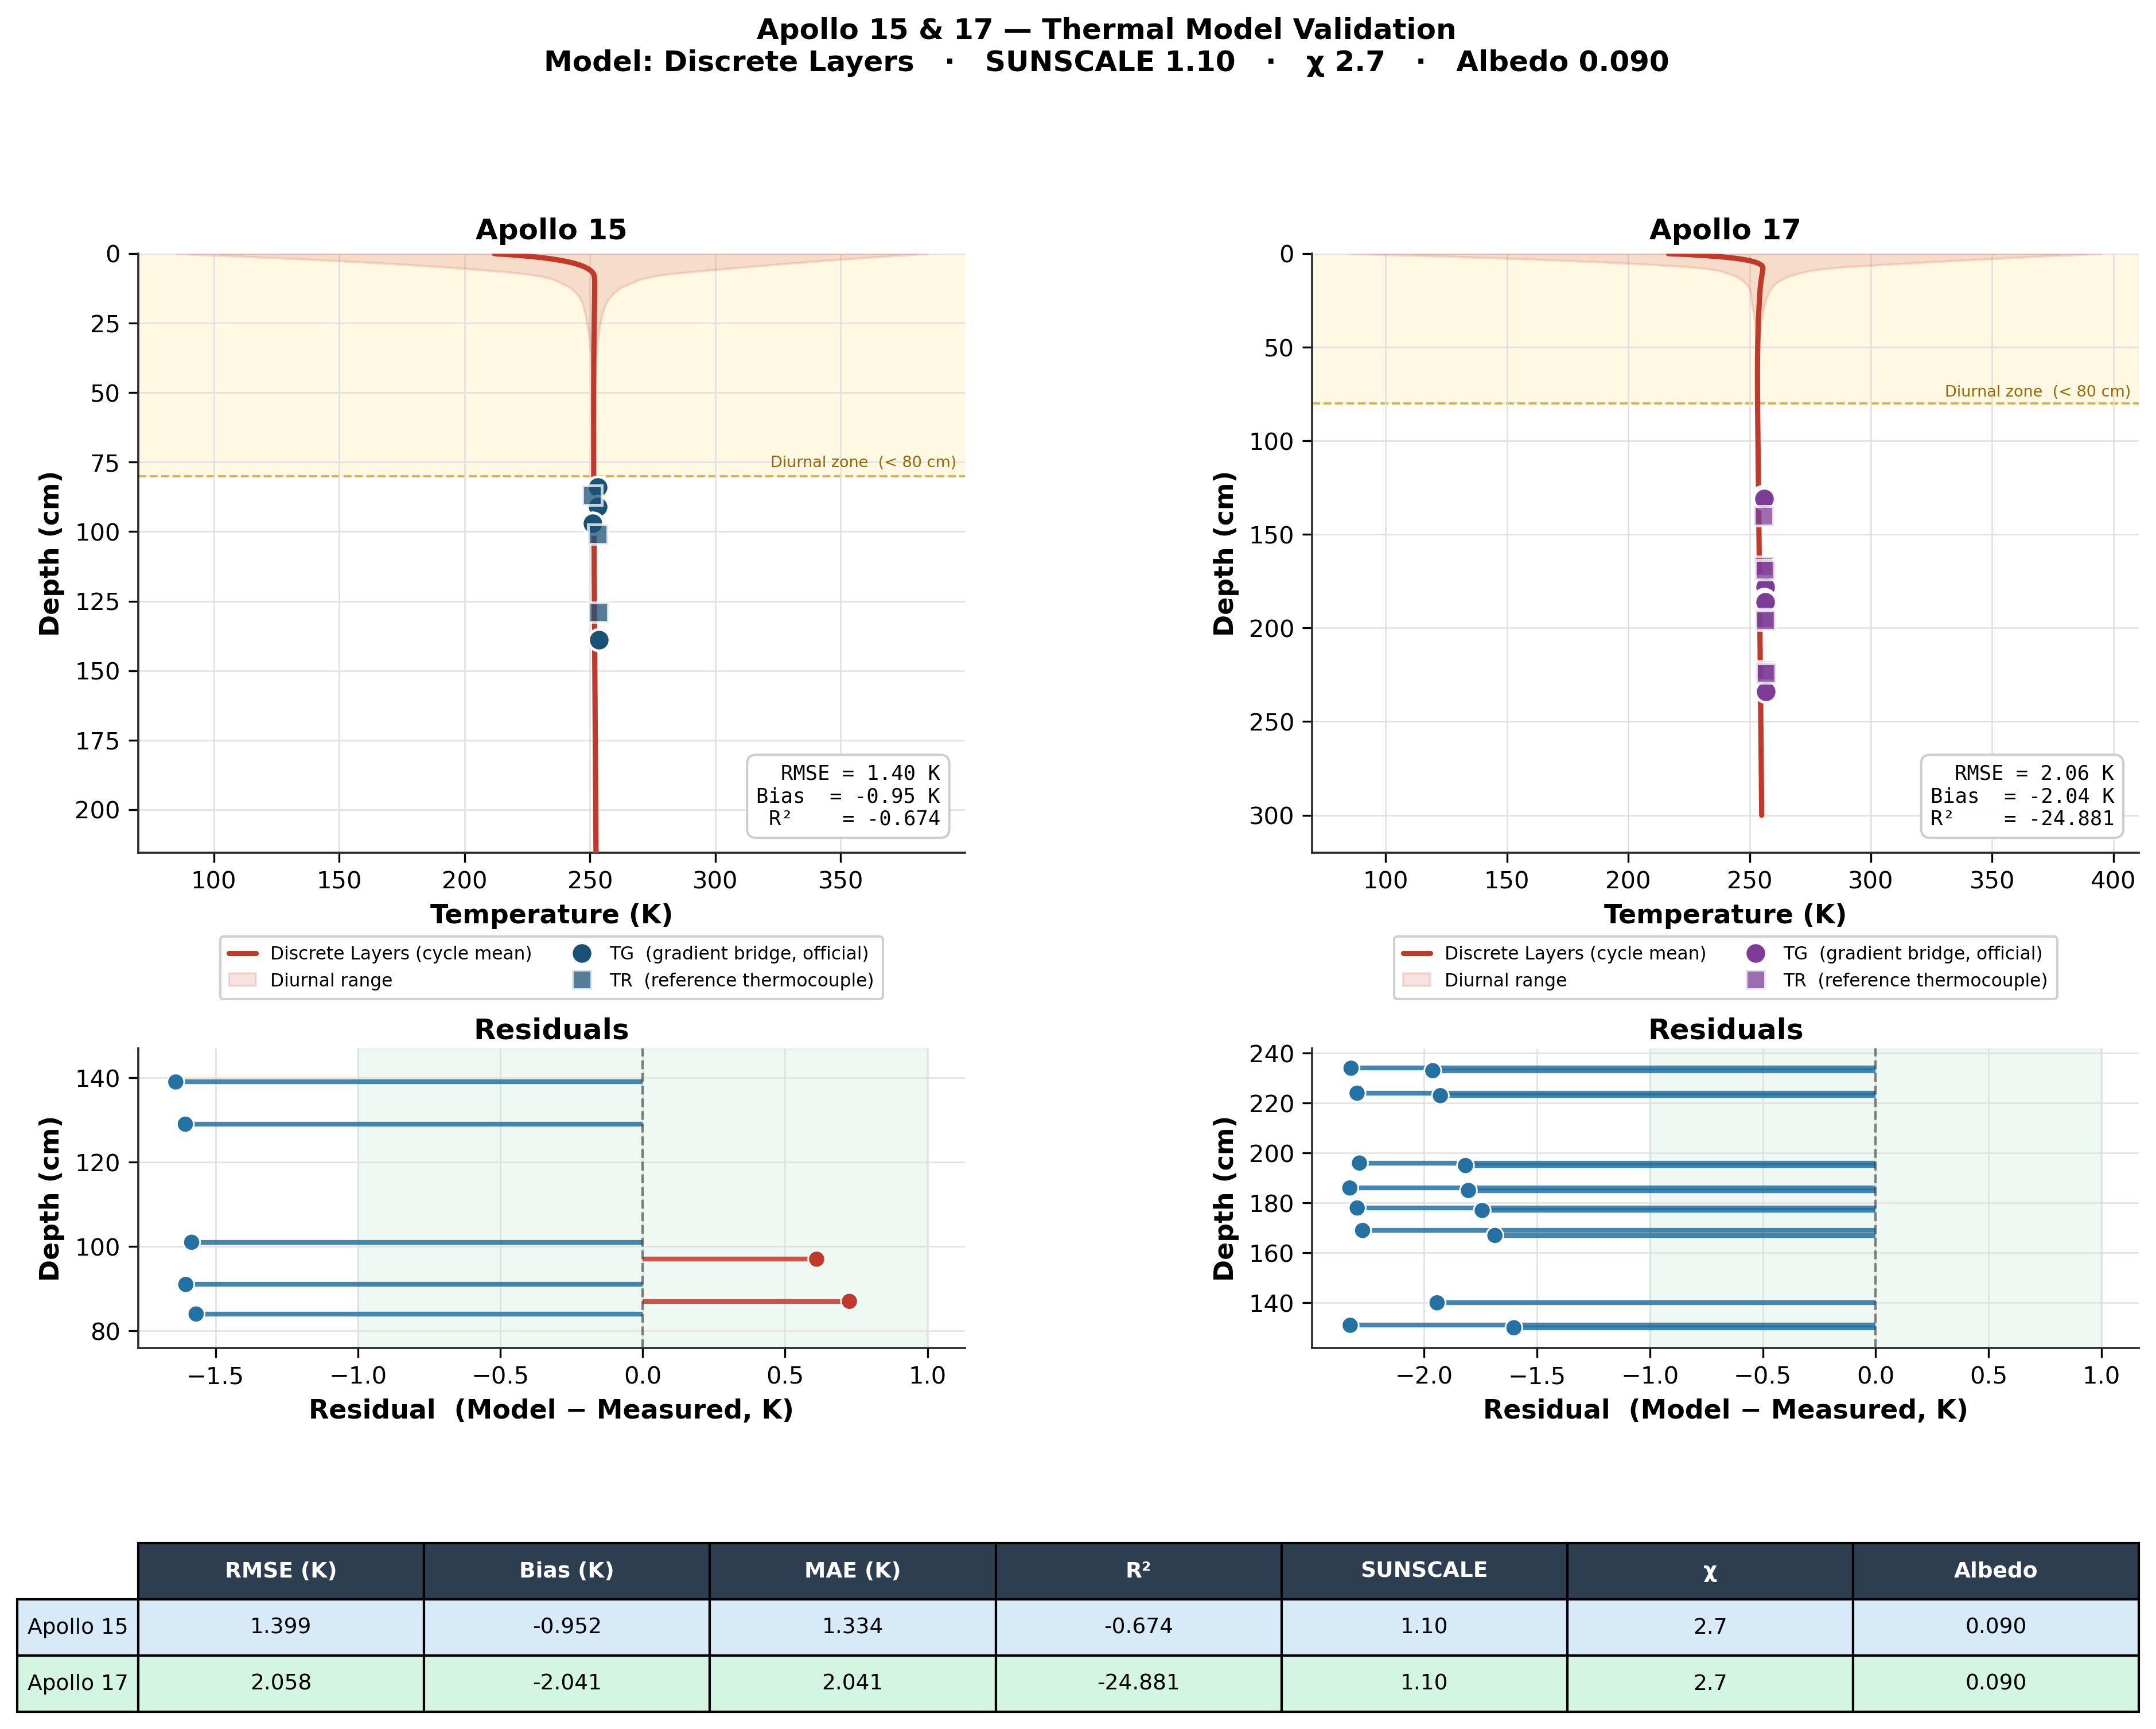
\includegraphics[width=\textwidth]{figures/08_dual_apollo_comparison.png}
  \caption{Model mean temperature profiles vs.\ Apollo HFE thermocouple
    data at Apollo~15 (left) and Apollo~17 (right).  Discrete model (red
    solid) and Hayne 2017 model (blue dashed).  Squares = TRR reference
    sensors; circles = TG gradient sensors.
    RMSE values are shown in the inset table.}
  \label{fig:comparison}
\end{figure}

Both models achieve RMSE $< 1.5$\,K against the Apollo data at
depths $\geq 80$\,cm, which is within the combined uncertainty of the
measurements and our simplified 1-D geometry.

%% ============================================================
\section{Geothermal Heat Flow}
%% ============================================================

The ultimate science goal is to measure how much heat the Moon releases
from its interior.  Figure~\ref{fig:heatflow} summarises the heat-flow
estimates from both sites.

\begin{figure}[H]
  \centering
  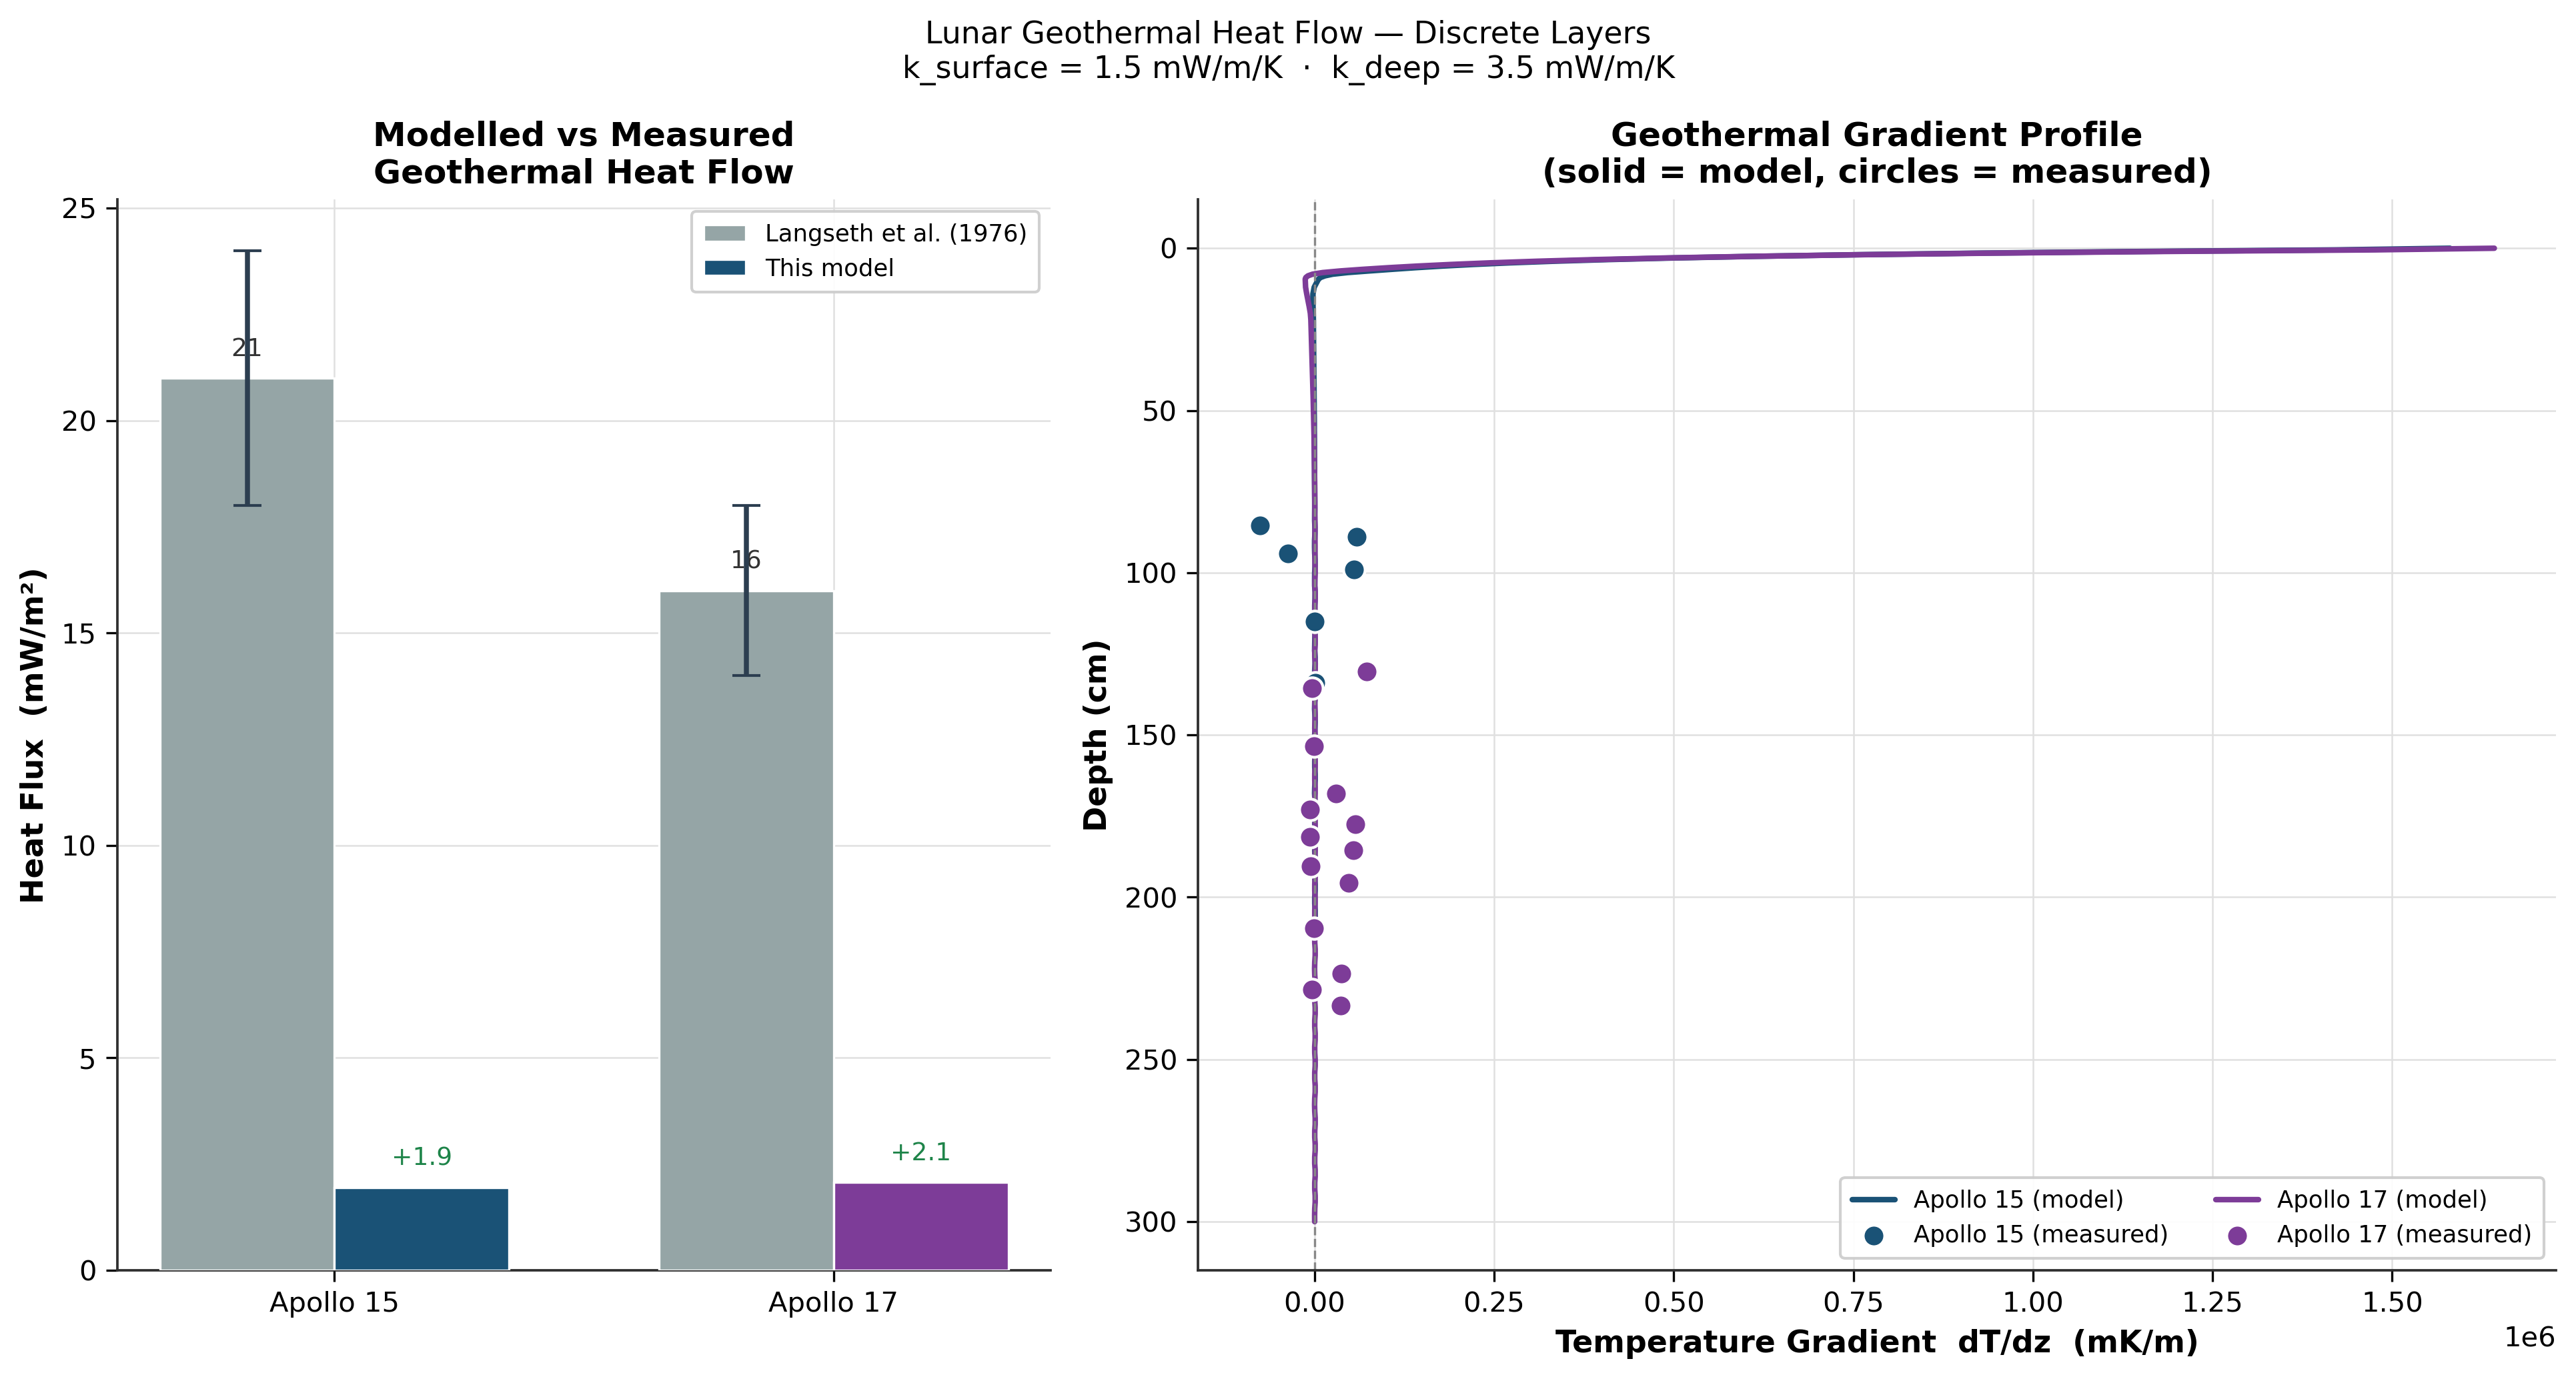
\includegraphics[width=0.85\textwidth]{figures/09_combined_heat_flow.png}
  \caption{Geothermal heat flow estimates.  Published Langseth et al.\
    (1976) values: $Q_{\text{A15}} = 21$\,mW/m$^2$,
    $Q_{\text{A17}} = 16$\,mW/m$^2$.  The model uses a shared value
    of 18\,mW/m$^2$.  For context, Earth's average heat flow is
    $\sim$65\,mW/m$^2$.  The Moon has cooled significantly.}
  \label{fig:heatflow}
\end{figure}

At 18\,mW/m$^2$, the Moon loses heat at roughly one-quarter the rate of
Earth per unit area.  This is consistent with the Moon having a smaller
radioactive element inventory and a largely solidified interior.

%% ============================================================
\section{Borestem Correction}
%% ============================================================

The Apollo probes were inserted into holes lined with a \textbf{fibreglass
bore stem} (a stiff tube to stop the borehole collapsing).  Fibreglass has
thermal conductivity $\approx 0.04$\,W/m/K, which is about 40$\times$ higher
than the surrounding surface regolith.

This acts like a thermal short circuit: heat flows along the probe body,
slightly distorting the temperature readings.  We apply a correction by
solving a 2-D axisymmetric steady-state model around the probe geometry.

\medskip
\textbf{Rule of thumb}: the borestem correction is small ($< 1$\,K) at
sensor depths $\geq 80$\,cm where the geothermal gradient dominates.  It
is largest and most uncertain at the shallowest sensors, which is one more
reason to exclude them from the main comparison.

%% ============================================================
\section{Numerical Method}
%% ============================================================

The model uses an \textbf{explicit finite-difference} scheme: the temperature
profile is discretised into $\sim$60 layers, and each layer's temperature is
updated at every time step using the temperatures of its neighbours.

\subsection{Stability criterion (Von Neumann)}

An explicit scheme can become unstable (temperatures blow up) if the time
step is too large.  The safe limit is:

\eqbox{
  $\Delta t < \dfrac{1}{2}\,\dfrac{(\Delta z)^2}{\alpha_{\max}}$,
  \quad $\alpha = \dfrac{k}{\rho\, c}$ (thermal diffusivity)
}

\noindent We use $\Delta t = 0.20 \times (\Delta t)_{\text{max}}$, a
comfortable safety margin.

\subsection{Spin-up}

The simulation runs for 7 complete lunar days (about 200 Earth days).
The first 6 days allow the near-surface temperatures to reach a
periodic steady state; only the final day is used for analysis.

%% ============================================================
\section{Key Parameters and References}
%% ============================================================

\begin{center}
\begin{tabular}{lll}
  \toprule
  Parameter & Value & Source \\
  \midrule
  Albedo $A$                     & 0.09        & Hayne et al.\ 2017 \\
  Emissivity $\varepsilon$       & 0.95        & Hayne et al.\ 2017 \\
  Radiative coefficient $\chi$   & 2.7         & Hayne et al.\ 2017 \\
  Geothermal flux $Q_{\text{b}}$ & 18 mW/m$^2$ & Langseth et al.\ 1976 \\
  Apollo 15 latitude             & 26.1\textdegree{}N  & NASA \\
  Apollo 17 latitude             & 20.2\textdegree{}N  & NASA \\
  Solar scale factor             & 1.10        & Calibrated to Apollo $T_{\text{mean}}$ \\
  \bottomrule
\end{tabular}
\end{center}

\subsection*{References}

\begin{itemize}[leftmargin=1.5em]
  \item Carrier, W.D., Olhoeft, G.R., \& Mendell, W. (1991). Physical
        properties of the lunar surface. \textit{Lunar Sourcebook},
        Chapter 9. Cambridge University Press.

  \item Hayne, P.O. et al.\ (2017). Global regolith thermophysical
        properties of the Moon from the Diviner Lunar Radiometer
        Experiment. \textit{JGR Planets}, 122, 2371--2400.
        \href{https://doi.org/10.1002/2017JE005387}{doi:10.1002/2017JE005387}

  \item Hemingway, B.S., Robie, R.A., \& Wilson, W.H. (1973).
        Specific heats of lunar soils, basalts, and breccias.
        \textit{Proc.\ Lunar Sci.\ Conf.\ 4th}, 2481--2487.

  \item Langseth, M.G., Keihm, S.J., \& Peters, K. (1976). Revised lunar
        heat-flow values. \textit{Proc.\ Lunar Sci.\ Conf.\ 7th},
        3143--3171.
\end{itemize}

\end{document}
